\documentclass[12pt]{article}

\usepackage[utf8]{inputenc}
\usepackage{Preambles/preamble}
\usepackage{listings}
\usepackage{url}
\usepackage{graphicx}


%~~~~~~~~~~~~~~~~~~~~~~~~~~~~~~~~~~~~~~~~~~~~~~~~~~~~~~~~~~~~~~

\begin{document}


\title{Project report: Coupling ScimBa and Feel++}

\firstauthor{Helya Amiri}
\firstemail{helya.amiri@etu.unistra.fr}
\secondauthor{Rayen Tlili}
\secondemail{rayen.tlili@etu.unistra.fr}
\supervisor{Christophe Prud'homme, Joubine Aghili}
\submitdate{\today}
\maketitle

\addtocounter{page}{-1}
\pagenumbering{roman}
\thispagestyle{empty}


\newpage
\doublespacing
\tableofcontents
\singlespacing
%~~~~~~~~~~~~~~~~~~~~~~~~~~~~~~~~~~~~~~~~~~~~~~~~~~~~~~~~~~~~~~
%Sections before Main Content of report

\newpage
\section*{Abstract}\label{Conventions}
\addcontentsline{toc}{subsection}{\textit{Abstract}}
\begin{frame}

    \item This project report details the integration efforts between ScimBa, emphasizing machine learning, and Feel++, known for its Galerkin methods in PDE solving. The aim is to establish seamless compatibility between the two libraries, fostering advanced computational techniques in scientific research. By combining machine learning with traditional PDE solvers, the project endeavors to propel computational science and engineering forward, enabling efficient data exchange and methodological synergy.
\end{frame}
\vspace{2em}

%~~~~~~~~~~~~~~~~~~~~~~~~~~~~~~~~~~~~~~~~~~~~~~~~~~~~~~~~~~~~~~
%Main Content sections start

\newpage
\pagenumbering{arabic}
\section*{Main Content}
\addcontentsline{toc}{part}{Main Content}

\section{Introduction} \label{Sec: Introduction}
This report presents the objectives, approach, and roadmap for the coupling of ScimBa and Feel++ libraries. ScimBa is a project aimed at integrating machine learning techniques with traditional scientific computing methods, while Feel++ is a C++ implementation of Galerkin methods for solving partial differential equations (PDEs). The coupling of these two libraries is expected to enhance their capabilities and enable researchers to solve complex scientific problems more effectively.


\section{Objectives}

This project endeavors to seamlessly unite the realms of ScimBa and Feel++, fostering a symbiotic relationship that optimally harnesses their individual strengths. At its core, the project aims to achieve the following objectives:

\begin{enumerate}
    \item \textbf{Strategic Analysis and Planning}: Delve into the functionalities of both ScimBa and Feel++ to discern strategic integration points. Develop a meticulous plan that charts the course for establishing loose coupling between these libraries, ensuring a harmonious blend of their capabilities.
    
    \item \textbf{Implementation Excellence}: Execute the envisioned integration strategy with precision and finesse. Implement a seamless coupling mechanism between ScimBa and Feel++, meticulously crafting methods to generate datasets within Feel++ and seamlessly integrate them into the ScimBa ecosystem.
    
    \item \textbf{Thorough Testing and Validation}: Subject the integrated system to rigorous testing and validation protocols, meticulously scrutinizing every aspect to ensure flawless communication between ScimBa and Feel++. Validate the efficacy of the coupling through the successful resolution of intricate scientific problems, affirming its transformative potential.
    
    \item \textbf{Comprehensive Documentation and Reporting}: Document the integration process meticulously, capturing interface definitions and communication protocols with meticulous detail. This documentation serves as a beacon for future endeavors, providing invaluable insights into the integration journey. Additionally, prepare a comprehensive report that encapsulates the project's outcomes, distilling key learnings and insights gleaned along the way.
\end{enumerate}

Through these objectives, the project aspires not merely to couple ScimBa and Feel++ but to forge a dynamic synergy that propels computational science into new realms of innovation and discovery.

%~~~~~~~~~~~~~~~~~~~~~~~~~~~~~~~~~~~~~~~~~~~~~~~~~~~~~~~~~~~~~~
%Github Roadmap

\newpage
\section{Roadmap}
\begin{figure}[H]
    \centering
    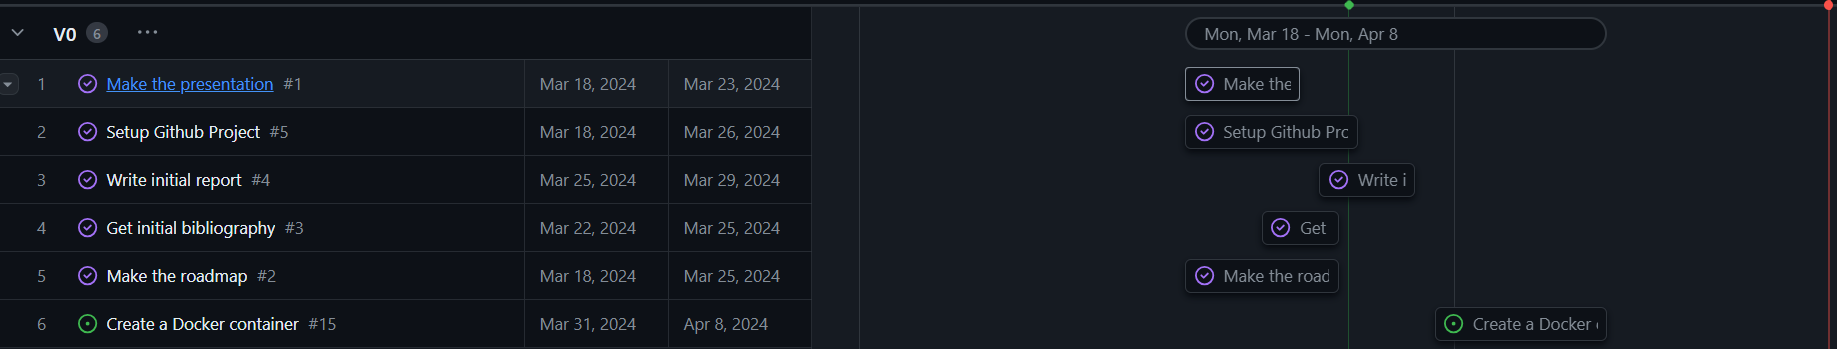
\includegraphics[width=0.7\textwidth]{images/roadmapV0.png}
    \captionsetup{font={scriptsize}}
    \caption{Roadmap for V0}
\end{figure}

\begin{figure}[H]
    \centering
    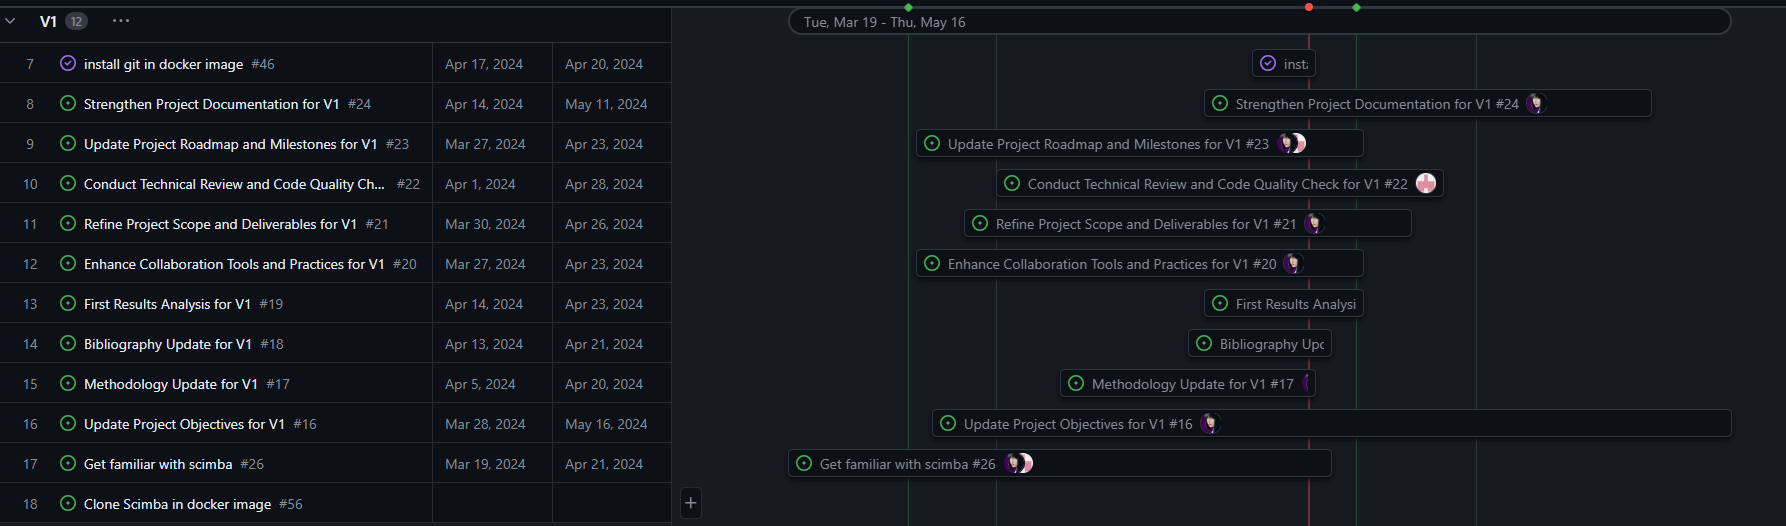
\includegraphics[width=0.7\textwidth]{images/roadmapV1.png}
    \captionsetup{font={scriptsize}}
    \caption{Roadmap for V1}
\end{figure}

\begin{figure}[H]
    \centering
    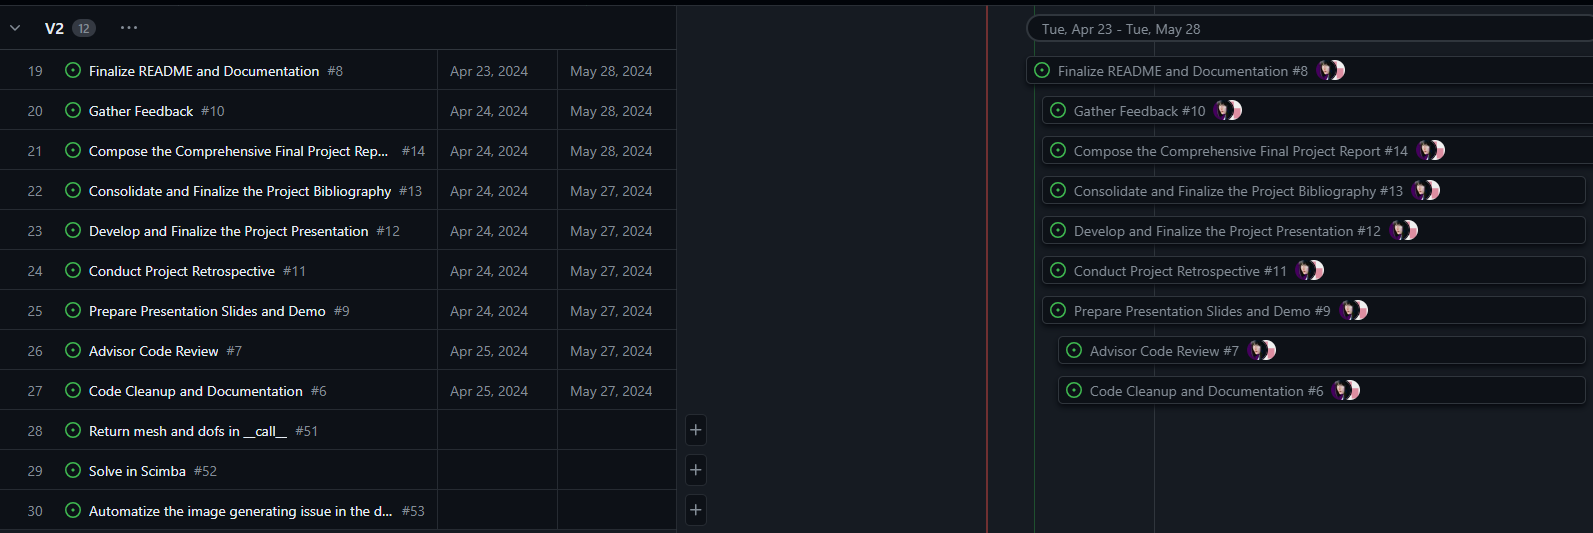
\includegraphics[width=0.7\textwidth]{images/roadmapV2.png}
    \captionsetup{font={scriptsize}}
    \caption{Roadmap for V2}
\end{figure}

%~~~~~~~~~~~~~~~~~~~~~~~~~~~~~~~~~~~~~~~~~~~~~~~~~~~~~~~~~~~~~~
\newpage
\section{Getting started}  

\subsection{Creating a Docker container}
Creating a Docker container and image for the project offers these key advantages:

\begin{enumerate}
    \item \textbf{Portability:} Run the project on any platform supporting Docker.
    \item \textbf{Isolation:} Avoid conflicts with other software on the host system.
    \item \textbf{Reproducibility:} Recreate the exact same environment whenever needed.
    \item \textbf{Dependency Management:} Package all dependencies within the Docker image.
    \\
\end{enumerate}


We're using Feel++ as the base for the Docker container, adding the requirements and dependencies for Scimba and PyTorch.

This Dockerfile contains the latest version of Feel++, Scimba, and PyTorch, and should be able to run these commands without error:
\\
\begin{lstlisting}[language=docker,caption={Dockerfile for Feel++, Scimba, and PyTorch},frame=single, backgroundcolor=\color{gray!10}, basicstyle=\footnotesize,rulecolor=\color{blue}, framexleftmargin=3pt, commentstyle=\color{mygreen}, keywordstyle=\color{blue}]
# Start with the Feel++ base image
FROM ghcr.io/feelpp/feelpp:jammy

# Set labels for metadata
LABEL maintainer="Helya Amiri <helya.amiri@etu.unistra.fr>,
      Rayen Tlili <rayen.tlili@etu.unistra.fr>"
LABEL description="Docker image with Feel++, Scimba, and PyTorch."

# Install PyTorch.
RUN pip3 install torch

# Copy the local Scimba directory to the container.
COPY scimba/ /scimba/

# Install Scimba and its dependencies
WORKDIR /scimba
USER root

RUN pip3 install .

# Set the default command to launch Python.
CMD ["python3"]
\end{lstlisting}


%~~~~~~~~~~~~~~~~~~~~~~~~~~~~~~~~~~~~~~~~~~~~~~~~~~~~~~~~~~~~~~
\newpage
\subsection{Exploring Feel++ toolboxes}

As of the first meeting with the project supervisors, we've taken a look at the different toolboxes Feel++ has to offer in Python:
\begin{frame}{}
    \begin{center}
        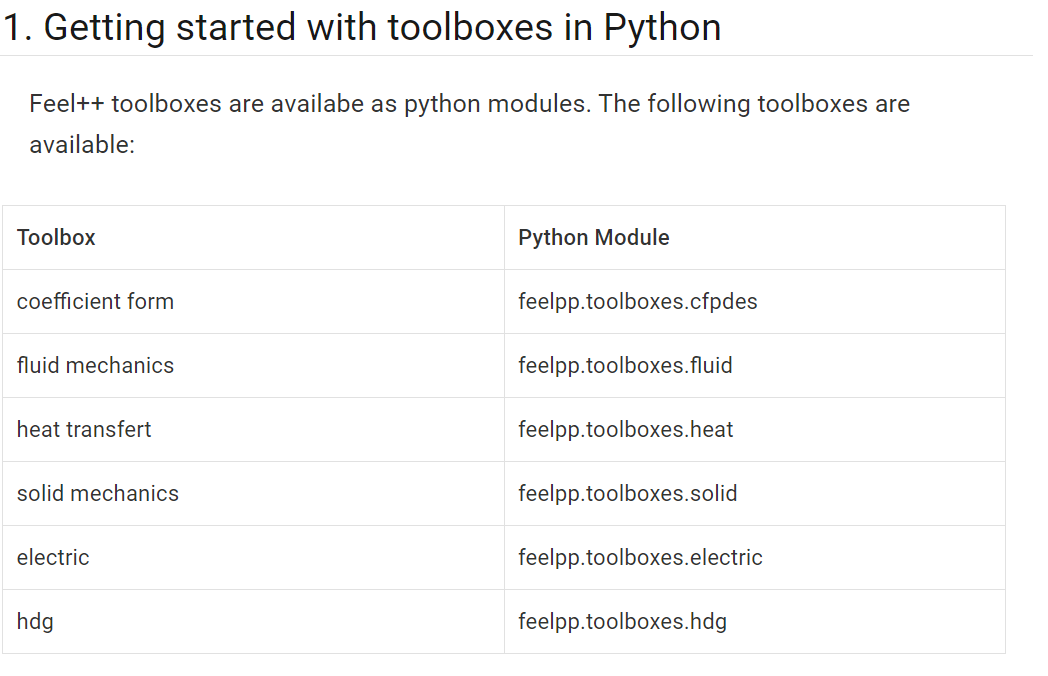
\includegraphics[width=0.7\textwidth]{images/pyfeelpptoolboxes.png}
    \end{center}
\end{frame}

An interesting toolbox to start with is the \textbf{Coefficient Form PDEs}:

%~~~~~~~~~~~~~~~~~~~~~~~~~~~~~~~~~~~~~~~~~~~~~~~~~~~~~~~~~~~~~~
\subsubsection{Coefficient Form Toolbox}

\begin{enumerate}
    \item \textbf{What are Coefficient Form PDEs?}: The coefficient forms in PDE (Partial Differential Equation) toolboxes encapsulate crucial properties like diffusion, convection, and reaction coefficients. These coefficients are vital for characterizing diverse PDEs such as elliptic, parabolic, or hyperbolic equations, each with its unique coefficient form.
    For instance, in the Poisson equation, a common elliptic equation, the coefficient form is often expressed as:
    \[
        -\nabla \cdot (c \nabla u) + au = f
    \]

    \begin{itemize}
        \item \(c\) : represents the diffusion coefficient,
        \item \(a\) : represents the reaction coefficient,
        \item \(u\) : is the unknown function, and
        \item \(f\) : is the source term.
    \end{itemize}
    
    PDE toolboxes, like Feel++, provide extensive features for managing coefficient forms in diverse PDEs. They simplify tasks such as defining coefficients, setting boundaries, discretizing problems, and employing numerical methods. These capabilities enable researchers and engineers to efficiently tackle complex PDEs, analyze various physical phenomena, and simulate real-world scenarios with ease.

    \item \textbf{System of PDEs}: A lot of PDE(s) can be written in a generic form, and depends mainly on the definition of coefficients. The generic form that we use is described by the following equation, to find \\
    \( u \) : \( \Omega \subset \mathbb{R}^d \longrightarrow \mathbb{R}^n \) with \( d = 2, 3 \) and \( n = 1 \) ( \( u \) is a scalar field) or \( n = d \) ( \( u \) is a vector field) such that
    \[
    d \frac{\partial u}{\partial t} + \nabla \cdot \left( -c \nabla u - \alpha u + \gamma \right) + \beta \cdot \nabla u + au = f \text{ in } \Omega
    \]
    \begin{itemize}
        \item \( d \) : damping or mass coefficient
        \item \( c \) : diffusion coefficient
        \item \( \alpha \) : conservative flux convection coefficient
        \item \( \gamma \) : conservative flux source term
        \item \( \beta \) : convection coefficient
        \item \( a \) : absorption or reaction coefficient
        \item \( f \) : source term
    \end{itemize}
    Parameters \( \mu \) may depend on the unknown \( u \) and on the space variable \( x \), time \( t \), and other unknowns \( u_1, \ldots, u_N \).

    \item \textbf{Coefficients}: We must also adhere to specific constraints regarding the shape of coefficients, outlined in the following table.
    \begin{figure}[H]
    \centering
    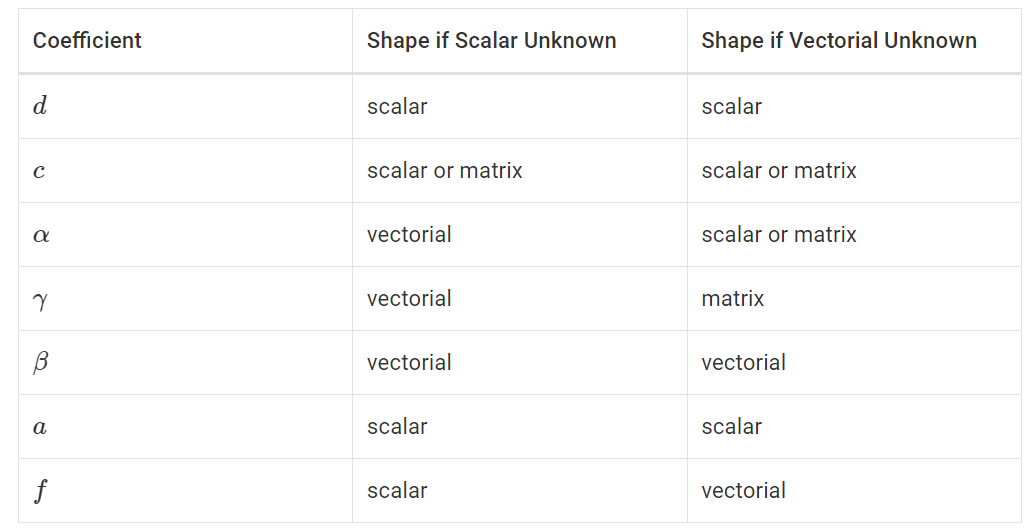
\includegraphics[width=0.6\textwidth]{images/coeff.png}
    \captionsetup{font={scriptsize}}
    \caption{Shape required by the coefficients}
    \end{figure}
    
\newpage
    \item \textbf{Initial Conditions}: Initial conditions specify the starting values for each unknown variable in the equations. These conditions can be defined using expressions or fields, as detailed in the JSON specifications.
    
    \item \textbf{ Boundary Conditions}: 
    \begin{itemize}
        \item Dirichlet
        \item Neumann
        \item Robin
    \end{itemize}
    
    \item \textbf{ Finite Element Approximation}  
    
    \item \textbf{Time scheme}:    
    \begin{itemize}
        \item Backward Differences Formula
        \item Theta scheme
    \end{itemize}  

    \item \textbf{ Stabilized finite element methods}  
    \begin{itemize}
        \item GaLS
        \item SUPG
        \item Coefficient form PDE toolbox        
    \end{itemize} 
 
\end{enumerate}
\end{frame}



%~~~~~~~~~~~~~~~~~~~~~~~~~~~~~~~~~~~~~~~~~~~~~~~~~~~~~~~~~~~~~~
\newpage

\section{Results}


%~~~~~~~~~~~~~~~~~~~~~~~~~~~~~~~~~~~~~~~~~~~~~~~~~~~~~~~~~~~~~~
\newpage

\section{Conclusion}


%~~~~~~~~~~~~~~~~~~~~~~~~~~~~~~~~~~~~~~~~~~~~~~~~~~~~~~~~~~~~~~
\newpage

\part*{Bibliography}
\addcontentsline{toc}{part}{\textit{Bibliography}}
\bibliographystyle{unsrt}
\bibliography{References.bib}


\begin{itemize}
    \item Feel++ Documentation: \url{https://docs.feelpp.org/user/latest/index.html}
    \item ScimBa Documentation: \url{https://sciml.gitlabpages.inria.fr/scimba/}
    \item Coupling : \url{https://en.wikipedia.org/wiki/Coupling_(computer_programming)}
    \item Using feel++:
    \url{https://www.cemosis.fr/events/course-solving-pdes-with-feel/}
    \item Feel++ documentation:
    \url{https://book.mso4sc.cemosis.fr/feelpp}

\end{itemize}

\end{document}

%Fin :)